\documentclass[]{article}
\usepackage{lmodern}
\usepackage{amssymb,amsmath}
\usepackage{ifxetex,ifluatex}
\usepackage{fixltx2e} % provides \textsubscript
\ifnum 0\ifxetex 1\fi\ifluatex 1\fi=0 % if pdftex
  \usepackage[T1]{fontenc}
  \usepackage[utf8]{inputenc}
\else % if luatex or xelatex
  \ifxetex
    \usepackage{mathspec}
  \else
    \usepackage{fontspec}
  \fi
  \defaultfontfeatures{Ligatures=TeX,Scale=MatchLowercase}
\fi
% use upquote if available, for straight quotes in verbatim environments
\IfFileExists{upquote.sty}{\usepackage{upquote}}{}
% use microtype if available
\IfFileExists{microtype.sty}{%
\usepackage[]{microtype}
\UseMicrotypeSet[protrusion]{basicmath} % disable protrusion for tt fonts
}{}
\PassOptionsToPackage{hyphens}{url} % url is loaded by hyperref
\usepackage[unicode=true]{hyperref}
\hypersetup{
            pdftitle={slapnap: Super LeArner Prediction of NAb Panels},
            pdfauthor={David Benkeser, Brian D. Williamson, Craig A. Magaret, Sohail Nizam, Peter B. Gilbert},
            pdfborder={0 0 0},
            breaklinks=true}
\urlstyle{same}  % don't use monospace font for urls
\usepackage[margin=1in]{geometry}
\usepackage{natbib}
\bibliographystyle{plainnat}
\usepackage{color}
\usepackage{fancyvrb}
\newcommand{\VerbBar}{|}
\newcommand{\VERB}{\Verb[commandchars=\\\{\}]}
\DefineVerbatimEnvironment{Highlighting}{Verbatim}{commandchars=\\\{\}}
% Add ',fontsize=\small' for more characters per line
\usepackage{framed}
\definecolor{shadecolor}{RGB}{248,248,248}
\newenvironment{Shaded}{\begin{snugshade}}{\end{snugshade}}
\newcommand{\KeywordTok}[1]{\textcolor[rgb]{0.13,0.29,0.53}{\textbf{#1}}}
\newcommand{\DataTypeTok}[1]{\textcolor[rgb]{0.13,0.29,0.53}{#1}}
\newcommand{\DecValTok}[1]{\textcolor[rgb]{0.00,0.00,0.81}{#1}}
\newcommand{\BaseNTok}[1]{\textcolor[rgb]{0.00,0.00,0.81}{#1}}
\newcommand{\FloatTok}[1]{\textcolor[rgb]{0.00,0.00,0.81}{#1}}
\newcommand{\ConstantTok}[1]{\textcolor[rgb]{0.00,0.00,0.00}{#1}}
\newcommand{\CharTok}[1]{\textcolor[rgb]{0.31,0.60,0.02}{#1}}
\newcommand{\SpecialCharTok}[1]{\textcolor[rgb]{0.00,0.00,0.00}{#1}}
\newcommand{\StringTok}[1]{\textcolor[rgb]{0.31,0.60,0.02}{#1}}
\newcommand{\VerbatimStringTok}[1]{\textcolor[rgb]{0.31,0.60,0.02}{#1}}
\newcommand{\SpecialStringTok}[1]{\textcolor[rgb]{0.31,0.60,0.02}{#1}}
\newcommand{\ImportTok}[1]{#1}
\newcommand{\CommentTok}[1]{\textcolor[rgb]{0.56,0.35,0.01}{\textit{#1}}}
\newcommand{\DocumentationTok}[1]{\textcolor[rgb]{0.56,0.35,0.01}{\textbf{\textit{#1}}}}
\newcommand{\AnnotationTok}[1]{\textcolor[rgb]{0.56,0.35,0.01}{\textbf{\textit{#1}}}}
\newcommand{\CommentVarTok}[1]{\textcolor[rgb]{0.56,0.35,0.01}{\textbf{\textit{#1}}}}
\newcommand{\OtherTok}[1]{\textcolor[rgb]{0.56,0.35,0.01}{#1}}
\newcommand{\FunctionTok}[1]{\textcolor[rgb]{0.00,0.00,0.00}{#1}}
\newcommand{\VariableTok}[1]{\textcolor[rgb]{0.00,0.00,0.00}{#1}}
\newcommand{\ControlFlowTok}[1]{\textcolor[rgb]{0.13,0.29,0.53}{\textbf{#1}}}
\newcommand{\OperatorTok}[1]{\textcolor[rgb]{0.81,0.36,0.00}{\textbf{#1}}}
\newcommand{\BuiltInTok}[1]{#1}
\newcommand{\ExtensionTok}[1]{#1}
\newcommand{\PreprocessorTok}[1]{\textcolor[rgb]{0.56,0.35,0.01}{\textit{#1}}}
\newcommand{\AttributeTok}[1]{\textcolor[rgb]{0.77,0.63,0.00}{#1}}
\newcommand{\RegionMarkerTok}[1]{#1}
\newcommand{\InformationTok}[1]{\textcolor[rgb]{0.56,0.35,0.01}{\textbf{\textit{#1}}}}
\newcommand{\WarningTok}[1]{\textcolor[rgb]{0.56,0.35,0.01}{\textbf{\textit{#1}}}}
\newcommand{\AlertTok}[1]{\textcolor[rgb]{0.94,0.16,0.16}{#1}}
\newcommand{\ErrorTok}[1]{\textcolor[rgb]{0.64,0.00,0.00}{\textbf{#1}}}
\newcommand{\NormalTok}[1]{#1}
\usepackage{longtable,booktabs}
% Fix footnotes in tables (requires footnote package)
\IfFileExists{footnote.sty}{\usepackage{footnote}\makesavenoteenv{long table}}{}
\usepackage{graphicx,grffile}
\makeatletter
\def\maxwidth{\ifdim\Gin@nat@width>\linewidth\linewidth\else\Gin@nat@width\fi}
\def\maxheight{\ifdim\Gin@nat@height>\textheight\textheight\else\Gin@nat@height\fi}
\makeatother
% Scale images if necessary, so that they will not overflow the page
% margins by default, and it is still possible to overwrite the defaults
% using explicit options in \includegraphics[width, height, ...]{}
\setkeys{Gin}{width=\maxwidth,height=\maxheight,keepaspectratio}
\IfFileExists{parskip.sty}{%
\usepackage{parskip}
}{% else
\setlength{\parindent}{0pt}
\setlength{\parskip}{6pt plus 2pt minus 1pt}
}
\setlength{\emergencystretch}{3em}  % prevent overfull lines
\providecommand{\tightlist}{%
  \setlength{\itemsep}{0pt}\setlength{\parskip}{0pt}}
\setcounter{secnumdepth}{5}
% Redefines (sub)paragraphs to behave more like sections
\ifx\paragraph\undefined\else
\let\oldparagraph\paragraph
\renewcommand{\paragraph}[1]{\oldparagraph{#1}\mbox{}}
\fi
\ifx\subparagraph\undefined\else
\let\oldsubparagraph\subparagraph
\renewcommand{\subparagraph}[1]{\oldsubparagraph{#1}\mbox{}}
\fi

% set default figure placement to htbp
\makeatletter
\def\fps@figure{htbp}
\makeatother


\title{\texttt{slapnap}: Super LeArner Prediction of NAb Panels}
\author{David Benkeser, Brian D. Williamson, Craig A. Magaret, Sohail Nizam,
Peter B. Gilbert}
\date{August 30, 2020}

\begin{document}
\maketitle

{
\setcounter{tocdepth}{2}
\tableofcontents
}
\section*{Welcome}\label{welcome}
\addcontentsline{toc}{section}{Welcome}

The \href{https://hub.docker.com/r/slapnap/slapnap}{\texttt{slapnap}}
container is a tool for using the Compile, Analyze and Tally NAb Panels
(CATNAP) database to develop predictive models of HIV-1 neutralization
sensitivity to one or several broadly neutralizing antibodies (bNAbs).

\begin{center}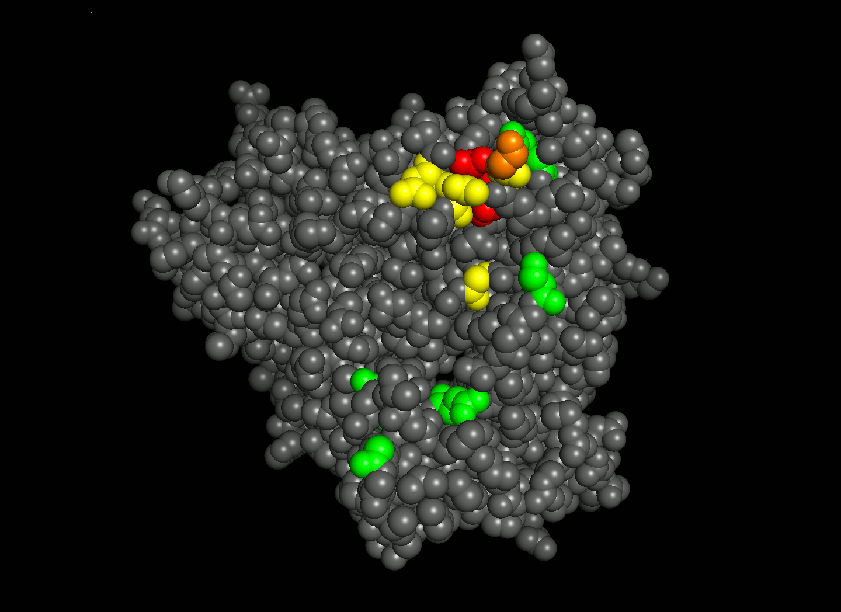
\includegraphics[width=0.7\linewidth]{gp120} \end{center}\begin{center}
Crystal structure of HIV-1 gp120 glycoprotein. Highlighted residues
indicating sites most-predictive of VRC01 neutralization resistance.
{[}@magaret2019prediction{]}
\end{center}

In its simplest form, \texttt{slapnap} can be used simply to access and
format data from CATNAP in a way that is usable for machine learning
analysis. However, the tool also offers fully automated and customizable
machine learning analyses based on up to five different neutralization
endpoints, complete with automated report generation to summarize
results and identify the most predictive features.

This document serves as the user manual for the \texttt{slapnap}
container. Here, we describe everything needed to utilize
\texttt{slapnap} and understand its output. The documentation is
organized into the following sections:

\begin{itemize}
\tightlist
\item
  Section \ref{sec:docker} provides a brief overview of Docker,
  including information on installing Docker and downloading the
  \texttt{slapnap} container.
\item
  Section \ref{sec:catnap} provides a brief overview of the CATNAP
  database and the specifics of how and when these data were accessed to
  build the \texttt{slapnap} container.
\item
  Section \ref{sec:runningcontainer} provides a detailed description of
  how to make calls to \texttt{slapnap} and all options that are
  available at run time to customize its behavior.
\item
  Section \ref{sec:examples} includes example calls to \texttt{slapnap}
  for accomplishing different tasks.
\item
  Section \ref{sec:methods} describes the methodology used by
  \texttt{slapnap} to generate and analyze data.
\item
  Section \ref{sec:report} describes the contents of the automated
  report generated by \texttt{slapnap}.
\item
  Section \ref{sec:data} provides a description of the analysis data set
  created by \texttt{slapnap}.
\end{itemize}

If you have any issues or questions about using \texttt{slapnap}, please
\href{https://github.com/benkeser/slapnap/issues}{file an issue} on
GitHub.

\section{Docker}\label{sec:docker}

Docker is a free platform for building containers. Containers are
standard units of software that package code and all its dependencies,
so that the code can be executed reliably irrespective of computing
environment. \texttt{slapnap} relies on machine learning implemented in
the \texttt{R} language and relies on several packages. Achieving full
reproducibility for such analyses is challenging in that it requires
synchronization across the specific version of \texttt{R} and dependent
packages. In other words, two users running two versions of \texttt{R}
or two versions of the same \texttt{R} package may arrive at different
output when running the same code. Containerization ensures that this
does not happen. Any two runs of \texttt{slapnap} with the same input
options will yield the same output every time.

\href{https://docs.docker.com/docker-for-windows/install/}{Installing
Docker} is necessary for running \texttt{slapnap}. While it is not
necessary for execution of the \texttt{slapnap} container, readers
interested in learning more about Docker should consult the
\href{https://docs.docker.com/get-started/}{Docker documentation} for
information about getting started using Docker.

Once Docker has been installed on your local computer, you can download
\texttt{slapnap} using the following command.

\begin{Shaded}
\begin{Highlighting}[]
\ExtensionTok{docker}\NormalTok{ pull slapnap/slapnap}
\end{Highlighting}
\end{Shaded}

This command pulls the image from
\href{https://hub.docker.com/}{DockerHub}. Once the image has been
downloaded, we are ready to learn about how to execute \texttt{slapnap}
jobs. The next section contains information on the source data used by
\texttt{slapnap}. Users familiar with the CATNAP data may wish to skip
directly to Section \ref{sec:opts}.

\section{CATNAP}\label{sec:catnap}

The
\href{https://www.hiv.lanl.gov/components/sequence/HIV/neutralization/index.html}{CATNAP
database} is a web server hosted by Los Alamos National Laboratory
\citep{yoon2015catnap}. The database integrates antibody neutralization
and HIV-1 sequence data from published studies. Neutralization is
measured in terms of half maximal inhibitory concentration (IC\(_{50}\))
and 80\% inhibitory concentration (IC\(_{80}\)). These measures of
neutralization against HIV envelope pseudoviruses are available for many
broadly neutralizing antibodies (bNAbs) and for some combination bNAbs.
Also available on each pseudovirus are amino acid (AA) sequence features
for the gp160 protein. These are detailed in Section \ref{sec:data}.

During each build of the \texttt{slapnap} container, all raw data are
downloaded from CATNAP. At run time, pseudovirus features are derived
and measured sensitivity outcomes are derived from the raw CATNAP
database files and merged into a \texttt{.csv} file that is used in
subsequent predictive analyses.

The CATNAP data are updated periodically. The data are downloaded into
the \texttt{slapnap} container at every build. The most recent build
occurred on August 30, 2020.

\section{\texorpdfstring{Running
\texttt{slapnap}}{Running slapnap}}\label{sec:runningcontainer}

To run the \texttt{slapnap} container, we make use of the
\href{https://docs.docker.com/engine/reference/run/}{\texttt{docker\ run}}
command. Note that administrator (\texttt{sudo}) privileges are needed
to execute this command. Additionally, note that \texttt{slapnap}
operates in UTC+0 time -- this will be important when inspecting the
files generated by \texttt{slapnap}.

There are several options that are necessary to include in this command
to control the behavior of \texttt{slapnap}. These are discussed in
separate subsections below.

\subsection{\texorpdfstring{\texttt{slapnap} run
options}{slapnap run options}}\label{sec:opts}

The user has control over many aspects of \texttt{slapnap}'s behavior.
These options are passed in using the \texttt{-e} option\footnote{This
  sets an environment variable in the container environment. These
  variables are accessed by the various \texttt{R} and \texttt{bash}
  scripts in the container to dictate how the container executes code.}.
Semi-colon separated strings are used to set options. For example, to
provide input for the option \texttt{option\_name}, we would used
\texttt{-e\ option\_name="a;semi-colon;separated;string"}. Note that
there are no spaces between the option name and its value and no spaces
after semi-colons in the separated list. See Section \ref{sec:examples}
for full syntax.

Each description below lists the default value that is assumed if the
option is not specified. Note that many of the default values are chosen
simply so that naive calls to \texttt{slapnap} compile quickly. Proper
values should be determined based on scientific context.

\textbf{-e options for \texttt{slapnap}}

\begin{itemize}
\tightlist
\item
  \textbf{\texttt{nab}}: A semicolon-separated list of bNAbs (default =
  \texttt{"VRC01"}). A list of possible bNAbs can be found
  \href{https://www.hiv.lanl.gov/components/sequence/HIV/neutralization/main.comp}{here}.
  If multiple bNAbs are listed, it is assumed that the analysis should
  be of estimated \texttt{outcomes} for a combination of bNAbs (see
  Section \ref{sec:outcomedefs} for details on how estimated outcomes
  for multiple bNAbs are computed).
\item
  \textbf{\texttt{outcomes}}: A semicolon-separated string of outcomes
  to include in the analysis. Possible values are \texttt{"ic50"}
  (included in default), \texttt{"ic80"}, \texttt{"iip"},
  \texttt{"sens"} (included in default), \texttt{"estsens"},
  \texttt{"multsens"}. If only a single \texttt{nab} is specified, use
  \texttt{sens} to include a dichotomous endpoint. If multiple
  \texttt{nab}s are specified, use \texttt{estsens} and/or
  \texttt{multsens}. For detailed definitions of outcomes see Section
  \ref{sec:outcomedefs}.
\item
  \textbf{\texttt{sens\_thresh}} A numeric value defining the
  IC\(_{50}\) threshold for defining a sensitive versus resistant
  pseudovirus (default = 1). The dichotomous sensitivity/resistant
  \texttt{outcome}s are defined as the indicator that (estimated)
  IC\(_{50}\) is greater than or equal to \texttt{sens\_thresh}.
\item
  \textbf{\texttt{multsens\_nab}} A numeric value used for defining
  whether a pseudovirus is resistant to a multi-nAb cocktail. Only used
  if \texttt{multsens} is included in \texttt{outcome} and more than one
  \texttt{nab} is requested. The dichotomous \texttt{outcome}
  \texttt{multsens} is defined as the indicator that a virus has
  IC\(_{50}\) greater than \texttt{sens\_thresh} for at least
  \texttt{multsens\_nab} nAbs.
\item
  \textbf{\texttt{learners}}: A semicolon-separated string of machine
  learning algorithms to include in the analysis. Possible values
  include \texttt{"rf"} (random forest, default), \texttt{"xgboost"}
  (eXtreme gradient boosting), and \texttt{"lasso"} (elastic net). See
  Section \ref{sec:learnerdetails} for details on how tuning parameters
  are chosen. If more than one algorithm is included, then it is assumed
  that a cross-validated-based ensemble (i.e., a super learner) is
  desired (see Section \ref{sec:sldetails}).
\item
  \textbf{\texttt{cvtune}}: A boolean string (i.e., either
  \texttt{"TRUE"} or \texttt{"FALSE"} {[}default{]}) indicating whether
  the \texttt{learners} should be tuned using cross validation and a
  small grid search. Defaults to \texttt{"FALSE"}. If multiple
  \texttt{learners} are specified, then the super learner ensemble
  includes three versions of each of the requested \texttt{learners}
  with different tuning parameters.
\item
  \textbf{\texttt{cvperf}}: A boolean string (i.e., either
  \texttt{"TRUE"} or \texttt{"FALSE"} {[}default{]}) indicating whether
  the \texttt{learners} performance should be evaluated using cross
  validation. If \texttt{cvtune="TRUE"} or \texttt{learners} includes
  multiple algorithms, then nested cross validation is used to evaluate
  the performance of the cross validation-selected best value of tuning
  parameters for the specified algorithm or the super learner,
  respectively.
\item
  \textbf{\texttt{var\_thresh}}: A numeric string that defines a
  threshold for pre-screening features. If a single positive number, all
  binary features with fewer than \texttt{var\_thresh} 0's or 1's are
  removed prior to the specified \texttt{learner} training. If several
  values are included in \texttt{var\_thresh} and a single
  \texttt{learner} is specified, then cross-validation is used to select
  the optimal threshold. If multiple \texttt{learner}s are specified,
  then each \texttt{learner} is included in the super learner with
  pre-screening based on each value of \texttt{var\_thresh}.
\item
  \textbf{\texttt{nfolds}}: A numeric string indicating the number of
  folds to use in cross validation procedures (default = \texttt{"2"}).
\item
  \textbf{\texttt{importance\_grp}}: A semicolon-separated string
  indicating which group-level variable importance measures should be
  computed. Possible values are none \texttt{""} (default), marginal
  \texttt{"marg"}, conditional \texttt{"cond"}. See Section
  \ref{sec:biolimp} for details on these measures.
\item
  \textbf{\texttt{importance\_ind}}: A semicolon-separated string
  indicating which individual-level variable importance measures should
  be computed. Possible values are none \texttt{""} (default),
  learner-level \texttt{"pred"}, marginal \texttt{"marg"} and
  conditional \texttt{"cond"}. The latter two take significant
  computation time to compute.
\item
  \textbf{\texttt{same\_subset}} If \texttt{"FALSE"} (default) all data
  available for each outcome will be used in the analysis. If
  \texttt{"TRUE"}, when multiple \texttt{outcomes} are requested, the
  data will be subset to just those sequences that have all measured
  \texttt{outcome}, and, if \texttt{iip} is requested, for which
  \texttt{iip} can be computed (i.e., measured IC\(_{50}\) and
  IC\(_{80}\) values are different). Thus, if \texttt{"TRUE"} all
  requested \texttt{outcomes} will be evaluated using the
  \texttt{same\_subset} of the CATNAP data.
\item
  \textbf{\texttt{report\_name}}: A string indicating the desired name
  of the output report (default =
  \texttt{report\_{[}\_-separated\ list\ of\ nabs{]}\_{[}date{]}.html}).
\item
  \textbf{\texttt{return}}: A semicolon-separated string of the desired
  output. Possible values are \texttt{"report"} (default),
  \texttt{"learner"} for a \texttt{.rds} object that contains the
  algorithm for each endpoint trained using the full analysis data,
  \texttt{"data"} for the analysis dataset, \texttt{"figures"} for all
  figures from the report, and \texttt{"vimp"} for variable importance
  objects.
\item
  \textbf{\texttt{view\_port}}: A boolean string indicating whether the
  compiled report should be made viewable on \texttt{localhost} (default
  \texttt{"FALSE"}). If \texttt{"TRUE"} then \texttt{-p} option should
  be used in the \texttt{docker\ run} command to identify the port. See
  example in Section \ref{sec:webbrowse} for details.
\end{itemize}

\subsection{Returning output}\label{returning-output}

At the end of a \texttt{slapnap} run, user-specified output will be
saved (see option \texttt{return} in Section \ref{sec:opts}). To
retrieve these files from the container, there are two options: mounting
a local directory (Section \ref{sec:mounting}) or, if the report is the
\textbf{only} desired output, viewing and saving the report in a web
browser (Section \ref{sec:viewreport}).

\subsubsection{Mounting a local directory}\label{sec:mounting}

To \href{https://docs.docker.com/storage/bind-mounts/}{mount} a local
directory to the output directory in the container
(\texttt{/home/output/}), use the \texttt{-v} option. Any items saved to
the output directory in the container (file path in the container
\texttt{/home/output/}) will be available in the mounted directory.
Conversely, all files in the mounted local directory will be visible to
programs running inside the container.

Suppose \texttt{/path/to/local/dir} is the file path on a local computer
in which we wish to save the output files from a \texttt{slapnap} run. A
\texttt{docker\ run} of \texttt{slapnap} would include the option
\texttt{-v\ /path/to/local/dir:/home/output}. After a run completes, the
requested output should be viewable in \texttt{/path/to/local/dir}. See
Section \ref{sec:examples} for full syntax.

To avoid possible naming conflicts and file overwrites in the mounted
directory, \textbf{we recommend mounting an empty directory} to store
the output.

Widows users need to
\href{https://docs.docker.com/docker-for-windows/troubleshoot/\#volume-mounting-requires-shared-drives-for-linux-containers}{enable
shared drives} by clicking
\texttt{Settings\ \textgreater{}\ Shared\ Drives} in the Docker Desktop
Daemon and sharing the drive that contains \texttt{path/to/local/dir}.

\subsubsection{Viewing report in browser}\label{sec:viewreport}

An alternative option to mounting local directories for viewing and
downloading the report is to set the \texttt{view\_port} option to
\texttt{"TRUE"} and open a port to the container via the \texttt{-p}
option in the \texttt{docker\ run} statement. In this case, rather than
exiting upon completion of the analysis, the container will continuing
to run and broadcast the compiled report to \texttt{localhost} at the
specified port (see examples below). The report can be downloaded from
the web browser directly in this way.

\section{Examples}\label{sec:examples}

\subsection{\texorpdfstring{Basic call to
\texttt{slapnap}}{Basic call to slapnap}}\label{basic-call-to-slapnap}

A call to \texttt{slapnap} with all default options can be run using the
following command.

\begin{Shaded}
\begin{Highlighting}[]
\ExtensionTok{docker}\NormalTok{ run -v /path/to/local/dir:/home/output slapnap/slapnap}
\end{Highlighting}
\end{Shaded}

Note that this call mounts the local directory
\texttt{path/to/local/dir} to receive output from the container (see
Section \ref{sec:mounting}).

When this command is executed, messages will print to indicate the
progress of the container. The first message will report the name of the
log file, which will appear in \texttt{/path/to/local/dir} (note that
the name of the log file is based on the current time, which is in
UTC+0). The container will then compile an analytic data set from the
CATNAP database for the default bNAb (VRC01), train the default learner
(random forest \citep{breiman2001}) for the default outcomes
(\texttt{ic50} and \texttt{sens}), evaluate its performance using
two-fold (default for \texttt{nfolds}) cross validation, and compile a
report detailing the results, and place the compiled report in
\texttt{path/to/local/dir} (note that the default name of the report is
based on the current time, which is in UTC+0).

\subsection{Viewing report in browser}\label{sec:webbrowse}

To have the results viewable in a web browser execute the following
command\footnote{In this command, we use the escape character
  \texttt{\textbackslash{}} to break the command over multiple lines,
  which will work on Linux and Mac OS. In Windows Command Prompt, the
  equivalent escape character is \texttt{\^{}}; in Windows Powershell,
  the equivalent escape character is \texttt{\textasciigrave{}}. In all
  cases, take care not to include a space after the escape character.}.

\begin{Shaded}
\begin{Highlighting}[]
\ExtensionTok{docker}\NormalTok{ run -v /path/to/local/dir:/home/output \textbackslash{}}
\NormalTok{           -e view_port=}\StringTok{"TRUE"}\NormalTok{ -p 80:80 \textbackslash{}}
\NormalTok{           slapnap/slapnap}
\end{Highlighting}
\end{Shaded}

This command opens port 80 on the container. Once the report has been
compiled, the container will not close down automatically. Instead it
will continue to run, broadcasting the report to port 80. Open a web
browser on your computer and navigate to \texttt{localhost:80} and you
should see the compiled report. Many web browsers should allow
downloading of the report (e.g., by right-clicking and selecting save
\texttt{Save\ As...}).

The container will continue to run until you tell it to \texttt{stop}.
To do that, retrieve the container ID by executing
\texttt{docker\ container\ ps}\footnote{To execute this command, you
  will need to hit \texttt{control\ +\ c} to return to the command
  prompt in the current shell or open a new shell. Alternatively, you
  could add the \texttt{-d} option to the \texttt{docker\ run} command,
  which will run the container in
  \href{https://docs.docker.com/engine/reference/run/\#detached-vs-foreground}{detached
  mode}.}. Copy the ID of the running container, which will be a string
of numbers and letters (say \texttt{a1b2c3d4}) and then execute
\texttt{docker\ stop\ a1b2c3d4} to shut down the container.

Note that in the above command, we have still mounted a local directory,
which may be considered best practice in case other output besides the
report is desired to be returned.

\subsection{Super learning}\label{super-learning}

If multiple \texttt{learner}s are specified, then a super learner
ensemble \citep{vanderlaan2007} is constructed based on the requested
\texttt{learner}s and a predictor that simply returns the empirical
average of the outcome (i.e., ignores all features entirely). In the
following command, we construct an ensemble based on a random forest
\citep{breiman2001} and elastic net \citep{zou2005}. Note that the
execution time for super learners can be considerably greater than for
single \texttt{learner}s because of the extra layer of cross validation
needed to construct the ensemble.

\begin{Shaded}
\begin{Highlighting}[]
\ExtensionTok{docker}\NormalTok{ run -v /path/to/local/dir:/home/output \textbackslash{}}
\NormalTok{           -e learners=}\StringTok{"rf;lasso"}\NormalTok{ \textbackslash{}}
\NormalTok{           slapnap/slapnap}
\end{Highlighting}
\end{Shaded}

For specific details on the super learner algorithms implemented in
\texttt{slapnap}, see Section \ref{sec:sldetails}.

\subsection{Train an algorithm}\label{train-an-algorithm}

The previous commands train learners and evaluate their performance
using cross validation. However, at times we may wish only to use
\texttt{slapnap} to train a particular algorithm, while avoiding the
additional computational time associated with evaluating its
cross-validated performance and compiling a report. We show an example
of this below using sensitivity as the outcome.

\begin{Shaded}
\begin{Highlighting}[]
\ExtensionTok{docker}\NormalTok{ run -v /path/to/local/dir:/home/output \textbackslash{}}
\NormalTok{           -e learners=}\StringTok{"rf"}\NormalTok{ \textbackslash{}}
\NormalTok{           -e return=}\StringTok{"learner"}\NormalTok{ \textbackslash{}}
\NormalTok{           -e cvperf=}\StringTok{"FALSE"}\NormalTok{ \textbackslash{}}
\NormalTok{           -e outcomes=}\StringTok{"sens"}\NormalTok{ \textbackslash{}}
\NormalTok{           slapnap/slapnap}
\end{Highlighting}
\end{Shaded}

After completion of this run, \texttt{learner\_sens.rds} will appear in
\texttt{/path/to/local/dir} that contains an \texttt{R} object of class
\texttt{ranger} (the \texttt{R} package used by \texttt{slapnap} to fit
random forests). You can confirm this from the command line by executing

\begin{Shaded}
\begin{Highlighting}[]
\ExtensionTok{Rscript}\NormalTok{ -e }\StringTok{"learner <- readRDS('/path/to/local/dir/learner_sens.rds'); class(learner)"}
\end{Highlighting}
\end{Shaded}

\subsection{Pull and clean data}\label{pull-and-clean-data}

The \texttt{slapnap} container can also be used to return cleaned CATNAP
data suitable for analyses not supported by the \texttt{slapnap}
pipeline. In this case, the container avoids training machine learning
algorithms and report generation, returning a data set and associated
documentation. In the following call, \texttt{return} only includes
\texttt{"data"}; thus, options pertaining to the machine learning
portions of \texttt{slapnap} are essentially ignored by
\texttt{slapnap}. The inputted \texttt{outcomes} are also irrelevant, as
all \texttt{outcomes} are included in the resultant data set.

\begin{Shaded}
\begin{Highlighting}[]
\ExtensionTok{docker}\NormalTok{ run -v /path/to/local/dir:/home/output \textbackslash{}}
\NormalTok{           -e return=}\StringTok{"data"}\NormalTok{ \textbackslash{}}
\NormalTok{           slapnap/slapnap}
\end{Highlighting}
\end{Shaded}

Note that the data set returned by \texttt{slapnap} contains the
\texttt{outcomes} used by \texttt{slapnap}; in other words, (estimated)
IC\(_{50}\), (estimated) IC\(_{80}\), and IIP are all log-transformed
(see Section \ref{sec:outcomedefs} for more details).

\subsection{Interactive sessions}\label{interactive-sessions}

To simply enter the container and poke around, use an interactive
session by including \texttt{-it} and overriding the container's
entry-point.

\begin{Shaded}
\begin{Highlighting}[]
\ExtensionTok{docker}\NormalTok{ run -it slapnap/slapnap /bin/bash}
\end{Highlighting}
\end{Shaded}

This will enter you into the container in a bash terminal prior to any
portions of the analysis being run. This may be useful for exploring the
file structure, examining versions of \texttt{R} packages that are
included in the container, etc.

To enter the container interactively \emph{after} the analysis has run,
you can execute the following commands. Here we add the \texttt{-d}
option to start the container in
\href{https://docs.docker.com/engine/reference/run/\#detached--d}{detached
mode}.

\begin{Shaded}
\begin{Highlighting}[]
\ExtensionTok{docker}\NormalTok{ run -d -p 80:80 -e view_port=}\StringTok{"TRUE"}\NormalTok{ slapnap/slapnap}

\CommentTok{# ...wait for analysis to finish...}

\CommentTok{# use this command to enter the container}
\ExtensionTok{docker}\NormalTok{ exec -it /bin/bash}
\end{Highlighting}
\end{Shaded}

To close the interactive session type \texttt{exit} at the container
command prompt and hit \texttt{Return}. This will close the container
and stop its running.

\section{Methods}\label{sec:methods}

\subsection{Outcomes}\label{sec:outcomedefs}

\subsubsection{Single bNAb}\label{single-bnab}

If a single bNAb or combination of bNAbs that are measured directly in
the CATNAP data is requested (i.e., the \texttt{nab} option is a single
string of a single bNAb or measured combination of bNAbs from the CATNAP
database), then the possible outcomes are:

\begin{itemize}
\tightlist
\item
  \texttt{ic50} = \(\mbox{log}_{10}(\mbox{IC}_{50})\), where IC\(_{50}\)
  is the half maximal inhibitory concentration;
\item
  \texttt{ic80} = \(\mbox{log}_{10}(\mbox{IC}_{80})\), where IC\(_{80}\)
  is the 80\% maximal inhibitory concentration;
\item
  \texttt{iip} = \((-1)\mbox{log}_{10}(1 - \mbox{IIP})\), where IIP
  \citep[\citet{wagh2016optimal}]{shen2008dose} is the instantaneous
  inhibitory potential, computed as
  \[ \frac{10^m}{\mbox{IC$_{50}$}^m + 10^m} \ , \] where
  \(m = \mbox{log}_{10}(4) / (\mbox{log}_{10}(\mbox{IC}_{80}) - \mbox{log}_{10}(\mbox{IC}_{50}))\);
  and
\item
  \texttt{sens} = sensitivity: the binary indicator that IC\(_{50}\)
  \(<\) \texttt{sens\_thresh}, the user-specified sensitivity threshold.
\end{itemize}

\subsubsection{Multiple bNAbs}\label{multiple-bnabs}

If multiple bNAbs are requested (i.e., the \texttt{nab} option is a
semi-colon separated string of more than one bNAb from CATNAP), then the
possible \texttt{outcomes} that can be requested are:

\begin{itemize}
\tightlist
\item
  \texttt{ic50} = \(\mbox{log}_{10}(\mbox{estimated IC}_{50})\), where
  estimated IC\(_{50}\) is computed as follows: for \(J\) bNAbs,
  \[ \mbox{estimated IC}_{50} = \left( \sum_{j=1}^J \mbox{IC}_{50,j}^{-1} \right)^{-1} \ , \]
  where IC\(_{50,j}\) denotes the measured IC\(_{50}\) for antibody
  \(j\) \citep{wagh2016optimal};
\item
  \texttt{ic80} = \(\mbox{log}_{10}(\mbox{estimated IC}_{80})\), where
  estimated IC\(_{80}\) is computed as follows: for \(J\) bNAbs,
  \[ \mbox{estimated IC}_{80} = \left( \sum_{j=1}^J \mbox{IC}_{80,j}^{-1} \right)^{-1} \ , \]
  where IC\(_{80,j}\) denotes the measured IC\(_{80}\) for antibody
  \(j\) \citep{wagh2016optimal};
\item
  \texttt{iip} = \((-1)\mbox{log}_{10}(1 - \mbox{IIP})\), where IIP is
  computed as \[ \frac{10^m}{\mbox{estimated IC$_{50}$}^m + 10^m} \ , \]
  where
  \(m = \mbox{log}_{10}(4) / (\mbox{log}_{10}(\mbox{estimated IC}_{80}) - \mbox{log}_{10}(\mbox{estimated IC}_{50}))\);
  and
\item
  \texttt{estsens} = estimated sensitivity: the binary indicator that
  estimated IC\(_{50}\) (defined above) is less than
  \texttt{sens\_thresh}; and
\item
  \texttt{multsens} = multiple sensitivity: the binary indicator that
  measured IC\(_{50}\) is less than the sensitivity threshold
  (\texttt{sens\_thresh}) for a number of bNAbs defined by
  \texttt{multsens\_nab}.
\end{itemize}

\subsection{Learners}\label{sec:learnerdetails}

There are three possible \texttt{learners} available in
\texttt{slapnap}: random forests \citep{breiman2001}, as implemented in
the \texttt{R} package \texttt{ranger} \citep{rangerpkg}; elastic net
\citep{zou2005} as implemented in \texttt{glmnet} \citep{glmnetpkg}; and
boosted trees \citep{friedman2001, chen2016} as implemented in
\texttt{xgboost} \citep{xgboostpkg}.

For each \texttt{learner}, there is a \texttt{default} choice of tuning
parameters that is implemented if \texttt{cvtune="FALSE"}. If instead
\texttt{cvtune="TRUE"}, then there are several choices of tuning
parameters that are evaluated using \texttt{nfold} cross validation,
Table \ref{tab:learners}.

\begin{table}

\caption{\label{tab:learners}Labels for `learners` in report and description of their respective tuning parameters}
\centering
\begin{tabular}[t]{l|l}
\hline
`learner` & Tuning parameters\\
\hline
`rf\_default` & `mtry` equal to square root of number of predictors\\
\hline
`rf\_1` & `mtry` equal to one-half times square root of number of predictors\\
\hline
`rf\_2` & `mtry` equal to two times square root of number of predictors\\
\hline
`xgboost\_default` & maximum tree depth equal to 4\\
\hline
`xgboost\_1` & maximum tree depth equal to 2\\
\hline
`xgboost\_2` & maximum tree depth equal to 6\\
\hline
`xgboost\_3` & maximum tree depth equal to 8\\
\hline
`lasso\_default` & \$\textbackslash{}lambda\$ selected by 5-fold CV and \$\textbackslash{}alpha\$ equal to 0\\
\hline
`lasso\_1` & \$\textbackslash{}lambda\$ selected by 5-fold CV and \$\textbackslash{}alpha\$ equal to 0.25\\
\hline
`lasso\_2` & \$\textbackslash{}lambda\$ selected by 5-fold CV and \$\textbackslash{}alpha\$ equal to 0.5\\
\hline
`lasso\_3` & \$\textbackslash{}lambda\$ selected by 5-fold CV and \$\textbackslash{}alpha\$ equal to 0.75\\
\hline
\end{tabular}
\end{table}

Tuning parameters not mentioned in the table are set as follows:

\begin{itemize}
\tightlist
\item
  \texttt{rf}: \texttt{num.trees\ =\ 500}, \texttt{min.node.size\ =\ 5}
  for continuous outcomes and \texttt{=\ 1} for binary outcomes;
\item
  \texttt{xgboost}: \texttt{nrounds\ =\ 1000}, \texttt{eta\ =\ 0.1},
  \texttt{min\_child\_weight\ =\ 10}, objective =
  \texttt{binary:logistic} for binary outcomes and
  \texttt{objective=reg:squarederror} for continuous outcomes.
\end{itemize}

\subsection{Super learner}\label{sec:sldetails}

If multiple \texttt{learners} are specified, then a super learner
ensemble \citep{vanderlaan2007} is constructed using \texttt{nfold}
cross validation, as implemented in the \texttt{R} package
\texttt{SuperLearner} \citep{superlearnerpkg}. Specifically, the data
are randomly partitioned into \texttt{nfold} chunks of approximately
equal size. For binary outcomes, this partitioning is done in such a way
as to ensure an approximately even number of sensitive/resistant
pseudoviruses in each chunk. A so-called super learner \emph{library} of
candidate algorithms is constructed by including different
\texttt{learners}:

\begin{itemize}
\tightlist
\item
  the algorithm \texttt{mean}, which reports back the sample mean as
  prediction for all observations is always included;
\item
  if \texttt{cvtune="FALSE"} then the \texttt{default} version of each
  \texttt{learner} (Section \ref{sec:learnerdetails}) is included;
\item
  if \texttt{cvtune="TRUE"} then each choice of tuning parameters for
  the selected \texttt{learners} in Table \ref{tab:learners} is
  included.
\end{itemize}

The cross-validated risk of each algorithm in the library is computed.
For binary outcomes, mean negative log-likelihood loss is used; for
continuous outcomes, mean squared-error is used. The single algorithm
with the smallest cross-validated risk is reported as the
\texttt{cv\ selector} (also known as the \emph{discrete} super learner).
The super learner ensemble is constructed by selecting convex weights
(i.e., each algorithm is assigned a non-negative weight and the weights
sum to one) that minimize cross-validated risk.

When \texttt{cvperf="TRUE"} and a super learner is constructed, an
additional layer of cross validation is used to evaluate the predictive
performance of the super learner and of the \texttt{cv\ selector}.

\subsection{Variable importance}\label{variable-importance}

If \texttt{importance\_grp} or \texttt{importance\_ind} is specified,
variable importance estimates are computed based on the
\texttt{learners}. Both biological and prediction importance can be
obtained; we discuss each in the following two sections.

\subsubsection{Biological importance}\label{sec:biolimp}

Biological importance may be obtained by specifying
\texttt{importance\_grp}, \texttt{importance\_ind}, or both. We provide
two types of biological importance: marginal and conditional, accessed
by passing \texttt{"marg"} and \texttt{"cond"}, respectively, to one of
the importance variables. Both types of biological importance are based
on the population prediction potential of features
\citep{williamson2020}, as implemented in the \texttt{R} package
\texttt{vimp} \citep{vimppkg}. We measure prediction potential using
nonparametric \(R^2\) for continuous outcomes (i.e., IC\(_{50}\),
IC\(_{80}\), or IIP) and using the nonparametric area under the receiver
operating characteristic curve (AUC) for binary outcomes (i.e.,
sensitivity, estimated sensitivity, or multiple sensitivity). In both
marginal and conditional importance, we compare the population
prediction potential including the feature(s) of interest to the
population prediction potential excluding the feature(s) or interest;
this provides a measure of the biological importance of the feature(s).
The two types of biological importance differ only in the other
adjustment variables that we consider: conditional importance compares
the prediction potential of all features to the prediction potential of
all features excluding the feature(s) of interest, and thus importance
must be interpreted conditionally; whereas marginal importance compares
the prediction potential of the feature(s) of interest plus geographic
confounders to the prediction potential of the geographic confounders
alone.

Both marginal and conditional biological importance can be computed for
groups of features or individual features. The available feature groups
are detailed in Section \ref{sec:data}. Execution time may increase when
biological importance is requested, depending upon the other options
passed to \texttt{slapnap}: a separate \texttt{learner} (or super
learner ensemble) must be trained for each feature group (or individual
feature) of interest. Marginal importance tends to be computed more
quickly than conditional importance, but both types of importance
provide useful information about the population of interest and the
underlying biology.

If biological importance is requested, then point estimates, confidence
intervals, and p-values (for a test of the null hypothesis that the
biological importance is equal to zero) will be computed and displayed
for each feature or group of features of interest. All results are based
on first creating two independent splits of the data: the population
prediction potential including the feature(s) of interest is estimated
on one half of the data, while the population prediction potential
excluding the feature(s) of interest is estimated on the remaining half.
This ensures that the procedure has the desired type I error rate.

In the following command, we request marginal biological importance for
the feature groups defined in Section \ref{sec:data}. We do not specify
a super learner ensemble to reduce computation time; however, in most
problems we recommend an ensemble to protect against model
misspecification.

\begin{Shaded}
\begin{Highlighting}[]
\ExtensionTok{docker}\NormalTok{ run -v /path/to/local/dir:/home/output \textbackslash{}}
\NormalTok{           -e importance_grp=}\StringTok{"marg"}\NormalTok{ \textbackslash{}}
\NormalTok{           slapnap/slapnap}
\end{Highlighting}
\end{Shaded}

The raw \texttt{R} objects (saved as \texttt{.rds} files) containing the
point estimates, confidence intervals, and p-values for biological
importance can be saved by passing \texttt{"vimp"} to \texttt{return}.

\subsubsection{Predictive importance}\label{predictive-importance}

\texttt{learner}-level predictive importance may be obtained by
including \texttt{"pred"} in the \texttt{importance\_ind} option. If a
single \texttt{learner} is fit, then the predictive importance is the
\texttt{R} default for that type of learner:

\begin{itemize}
\tightlist
\item
  \texttt{rf}: the \texttt{impurity} importance from \texttt{ranger}
  \citep{rangerpkg} is returned. The impurity importance for a given
  feature is computed by taking a normalized sum of the decrease in
  impurity (i.e., Gini index for binary outcomes; mean squared-error for
  continuous outcomes) over all nodes in the forest at which a split on
  that feature has been conducted.
\item
  \texttt{xgboost}: the \texttt{gain} importance from \texttt{xgboost}
  \citep{xgboostpkg} is returned. Interpretation is essentially the same
  as for \texttt{rf}'s \texttt{impurity} importance.
\item
  \texttt{lasso}: the absolute value of the estimated regression
  coefficient at the cross-validation-selected \(\lambda\) is returned.
\end{itemize}

Note that these importance measures each have important limitations: the
\texttt{rf} and \texttt{xgboost} measures will tend to favor features
with many levels, while the \texttt{lasso} variable importance will tend
to favor features with few levels. Nevertheless, these commonly reported
measures can provide some insight into how a given learner is making
predictions.

If multiple \texttt{learners} are used, and thus a super learner is
constructed, then the importance measures for the \texttt{learner} with
the highest weight in the super learner are reported.

If a single \texttt{learner} is used, but \texttt{cvtune="TRUE"} then
importance measures for the \texttt{cv\ selector} are reported.

In the following command, we request predictive importance for a simple
scenario. Predictive importance is displayed for the top 15 features.

\begin{Shaded}
\begin{Highlighting}[]
\ExtensionTok{docker}\NormalTok{ run -v /path/to/local/dir:/home/output \textbackslash{}}
\NormalTok{           -e importance_ind=}\StringTok{"pred"}\NormalTok{ \textbackslash{}}
\NormalTok{           slapnap/slapnap}
\end{Highlighting}
\end{Shaded}

\section{Report}\label{sec:report}

The \texttt{slapnap} report consists of an executive summary followed by
results for each requested outcome.

The executive summary contains:

\begin{itemize}
\tightlist
\item
  descriptions of \texttt{outcomes} (including how any derived outcomes
  are generated);
\item
  descriptive statistics detailing the number of sequences extracted
  from CATNAP, the number of sequences with complete feature and outcome
  information, and the number of estimated sensitive and resistant
  sequences (defined based on sensitivity, estimated sensitivity, and/or
  multiple sensitivity);
\item
  a table describing the \texttt{learners} used to predict each outcome;
\item
  a table of cross-validated prediction performance for each outcome (if
  \texttt{cvperf\ =\ TRUE});
\item
  a table of ranked marginal biological prediction performance for each
  feature group and outcome (if \texttt{"marg"} is included in
  \texttt{importance\_grp}); and
\item
  a table of ranked conditional biological prediction performance for
  each feature group and outcome (if \texttt{"cond"} is included in
  \texttt{importance\_grp}).
\end{itemize}

The rest of the report is organized by outcome. Each of these sections
contains descriptive statistics including summaries of the distribution
of the outcome (raw and log-transformed) for each bNAb for continuous
outcomes and number sensitive/resistant for binary outcomes. Based on
the specific options passed to \texttt{slapnap}, the following
subsections may also be present:

\begin{itemize}
\tightlist
\item
  a table of super learner weights (Section \ref{sec:sldetails}) if an
  ensemble is used;
\item
  cross-validated prediction performance for the fitted learner (or
  super learner): figures showing cross-validated prediction performance
  (all outcomes), cross-validated receiver operating characteristic
  (ROC) curves (binary outcomes), and cross-validated predicted
  probabilities of resistance (binary outcomes); and
\item
  variable importance: biological importance (group and individual) and
  predictive importance.
\end{itemize}

Finally, if group biological importance is requested, then the variable
groups are displayed in a section immediately preceding the references.

\section{Data}\label{sec:data}

The analysis dataset includes neutralization outcomes for the requested
bNAb(s) and AA sequence features for the gp160 protein. The possible
outcomes are described in Section \ref{sec:outcomedefs}.

The additional groups of variables in the data include:

\begin{itemize}
\tightlist
\item
  \textbf{geographic information}: binary indicator variables describing
  the region of origin of each pseudovirus;
\item
  \textbf{subtype}: binary indicator variables denoting the HIV-1
  subtype for the given pseudovirus;
\item
  \textbf{AA sequence features}: binary indicator variables denoting
  presence or absence of a residue containing a specific AA at each
  HXB2-referenced site in gp160;
\item
  \textbf{viral geometry features}: length of Env, gp120, V2, V3, V5;
\item
  \textbf{numbers of sequons}: number of sequons in Env, gp120, V2, V3,
  V5; and
\item
  \textbf{numbers of cysteines}: number of cysteines in Env, gp120, V2,
  V3, V5.
\end{itemize}

\section{References}\label{sec:refs}

\bibliography{refs.bib}

\end{document}
